\chapter{Is every theorem provable?}\label{godelchap}

\begin{objectives} \label[objectives]{More-examples-of-uncomput}

\begin{itemize}
\tightlist
\item
  More examples of uncomputable functions that are not as tied to
  computation.
\item
  Gödel's incompleteness theorem - a result that shook the world of
  mathematics in the early 20th century.
\end{itemize}

\end{objectives}

\begin{quote}
\emph{``Take any definite unsolved problem, such as \ldots{} the
existence of an infinite number of prime numbers of the form
\(2^n + 1\). However unapproachable these problems may seem to us and
however helpless we stand before them, we have, nevertheless, the firm
conviction that their solution must follow by a finite number of purely
logical processes\ldots{}''}\\
\emph{``\ldots This conviction of the solvability of every mathematical
problem is a powerful incentive to the worker. We hear within us the
perpetual call: There is the problem. Seek its solution. You can find it
by pure reason, for in mathematics there is no ignorabimus.''}, David
Hilbert, 1900.
\end{quote}

\begin{quote}
\emph{``The meaning of a statement is its method of verification.''},
Moritz Schlick, 1938 (aka ``The verification principle'' of logical
positivism)
\end{quote}

The problems shown uncomputable in \cref{chapcomputable}, while natural
and important, still intimately involved NAND-TM programs or other
computing mechanisms in their definitions. One could perhaps hope that
as long as we steer clear of functions whose inputs are themselves
programs, we can avoid the ``curse of uncomputability''. Alas, we have
no such luck.

In this chapter we will see an example of a natural and seemingly
``computation free'' problem that nevertheless turns out to be
uncomputable: solving Diophantine equations. As a corollary, we will see
one of the most striking results of 20th century mathematics:
\emph{Gödel's Incompleteness Theorem}, which showed that there are some
mathematical statements (in fact, in number theory) that are
\emph{inherently unprovable}. We will actually start with the latter
result, and then show the former.


\begin{figure}
\centering
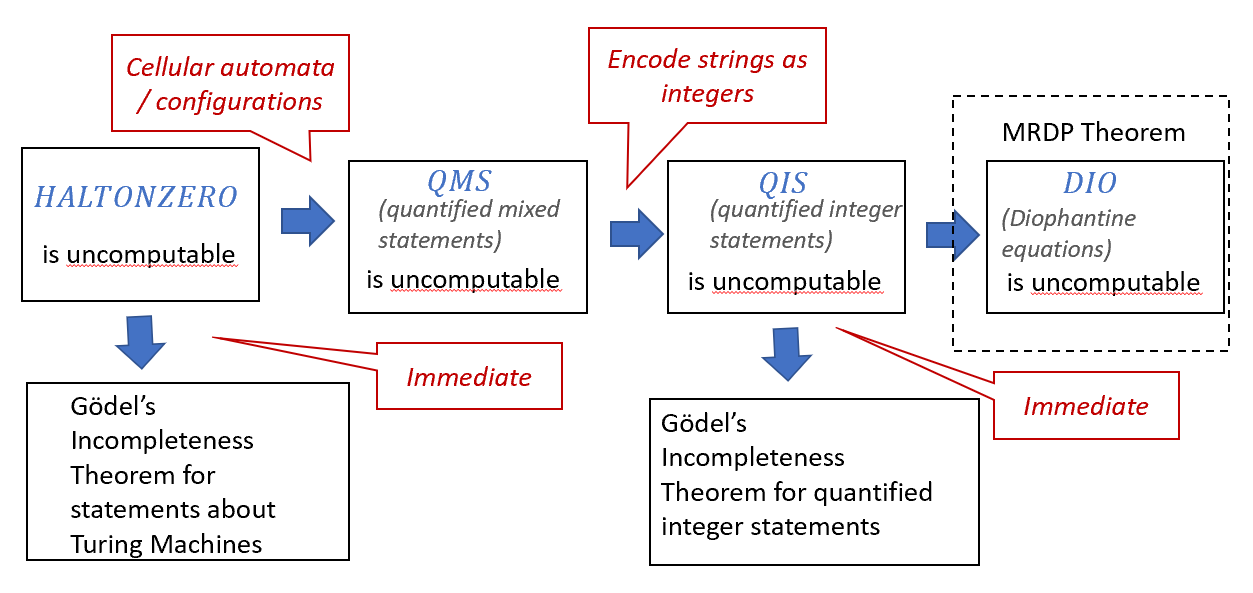
\includegraphics[width=\textwidth, height=0.25\paperheight, keepaspectratio]{../figure/godelstructure.png}
\caption{Outline of the results of this chapter. One version of Gödel's
Incompleteness Theorem is an immediate concsequence of the
uncomputability of the Halting problem. To obtain the theorem as
originally stated (for statements about the integers) we first prove
that the \(\ensuremath{\mathit{QMS}}\) problem of determining truth of
quantified statements involving both integers and strings is
uncomputable. We do so using the notion of \emph{Turing Machine
configurations} but there are alternative approaches to do so as well,
see \cref{alternativeproofs}.}
\label{godelstructurefig}
\end{figure}

\section{Hilbert's Program and Gödel's Incompleteness
Theorem}\label{godelproofdef}

\begin{quote}
\emph{``And what are these \ldots vanishing increments? They are neither
finite quantities, nor quantities infinitely small, nor yet nothing. May
we not call them the ghosts of departed quantities?''}, George Berkeley,
Bishop of Cloyne, 1734.
\end{quote}

The 1700's and 1800's were a time of great discoveries in mathematics
but also of several crises. The discovery of calculus by Newton and
Leibnitz in the late 1600's ushered a golden age of problem solving.
Many longstanding challenges succumbed to the new tools that were
discovered, and mathematicians got ever better at doing some truly
impressive calculations. However, the rigorous foundations behind these
calculations left much to be desired. Mathematicians manipulated
infinitesimal quantities and infinite series cavalierly, and while most
of the time they ended up with the correct results, there were a few
strange examples (such as trying to calculate the value of the infinite
series \(1-1+1-1+1+\ldots\)) which seemed to give out different answers
depending on the method of calculation. This led to a growing sense of
unease in the foundations of the subject which was addressed in the
works of mathematicians such as Cauchy, Weierstrass, and Riemann, who
eventually placed analysis on firmer foundations, giving rise to the
\(\epsilon\)'s and \(\delta\)'s that students taking honors calculus
grapple with to this day.

In the beginning of the 20th century, there was an effort to replicate
this effort, in greater rigor, to all parts of mathematics. The hope was
to show that all the true results of mathematics can be obtained by
starting with a number of axioms, and deriving theorems from them using
logical rules of inference. This effort was known as the \emph{Hilbert
program}, named after the influential mathematician David Hilbert.

Alas, it turns out the results we've seen dealt a devastating blow to
this program, as was shown by Kurt Gödel in 1931:

\hypertarget{godethmtakeone}{}
\begin{theorem}[Gödel's Incompleteness Theorem:  informal version] \label[theorem]{godethmtakeone}

For every sound proof system \(V\) for sufficiently rich mathematical
statements, there is a mathematical statement that is \emph{true} but is
not \emph{provable} in \(V\).

\end{theorem}

\subsection{Defining ``Proof Systems''}\label{godelproofsystemssec}

Before proving \cref{godethmtakeone}, we need to define ``proof
systems'' and even formally define the notion of a ``mathematical
statement''. In geometry and other areas of mathematics, proof systems
are often defined by starting with some basic assumptions or
\emph{axioms} and then deriving more statements by using \emph{inference
rules} such as the famous
\href{https://en.wikipedia.org/wiki/Modus_ponens}{Modus Ponens}, but
what axioms shall we use? What rules? We will use an extremely general
notion of proof systems, not even restricting ourselves to ones that
have the form of axioms and inference.

\paragraph{Mathematical statements.} At the highest level, a
mathematical statement is simply a piece of text, which we can think of
as a \emph{string} \(x\in \{0,1\}^*\). Mathematical statements contain
assertions whose truth does not depend on any empirical fact, but rather
only on properties of abstract objects. For example, the following is a
mathematical statement:\footnote{This happens to be a \emph{false}
  statement.}

\begin{quote}
\emph{``The number
\(2\),\(696\),\(635\),\(869\),\(504\),\(783\),\(333\),\(238\),\(805\),\(675\),\(613\),
\(588\),\(278\),\(597\),\(832\),\(162\),\(617\),\(892\),\(474\),\(670\),\(798\),\(113\)
is prime''.}
\end{quote}

Mathematical statements do not have to involve numbers. They can assert
properties of any other mathematical object including sets, strings,
functions, graphs and yes, even \emph{programs}. Thus, another example
of a mathematical statement is the following:\footnote{It is
  \href{https://goo.gl/Lx8HYv}{unknown} whether this statement is true
  or false.}

\begin{quote} \label[quote]{The-following-Python-func}

The following Python function halts on every positive integer \texttt{n}

\begin{code}
def f(n):
    if n==1: return 1
    return f(3*n+1) if n % 2 else f(n//2)
\end{code}

\end{quote}

\paragraph{Proof systems.} A \emph{proof} for a statement
\(x\in \{0,1\}^*\) is another piece of text \(w\in \{0,1\}^*\) that
certifies the truth of the statement asserted in \(x\). The conditions
for a valid proof system are:

\begin{enumerate}
\def\labelenumi{\arabic{enumi}.}
\item
  \emph{(Effectiveness)} Given a statement \(x\) and a proof \(w\),
  there is an algorithm to verify whether or not \(w\) is a valid proof
  for \(x\). (For example, by going line by line and checking that each
  line follows from the preceding ones using one of the allowed
  inference rules.)
\item
  \emph{(Soundness)} If there is a valid proof \(w\) for \(x\) then
  \(x\) is true.
\end{enumerate}

These are quite minimal requirements for a proof system. Requirement 2
(soundness) is the very definition of a proof system: you shouldn't be
able to prove things that are not true. Requirement 1 is also essential.
If there is no set of rules (i.e., an algorithm) to check that a proof
is valid then in what sense is it a proof system? We could replace it
with a system where the ``proof'' for a statement \(x\) is ``trust me:
it's true''.

We formally define proof systems as an algorithm \(V\) where
\(V(x,w)=1\) holds if the string \(w\) is a valid proof for the
statement \(x\). Even if \(x\) is true, the string \(w\) does not have
to be a valid proof for it (there are plenty of wrong proofs for true
statements such as \texttt{4=2+2}) but if \(w\) is a valid proof for
\(x\) then \(x\) must be true.

\hypertarget{proofsystemsdef}{}
\begin{definition}[Proof systems] \label[definition]{proofsystemsdef}

Let \(\mathcal{T} \subseteq \{0,1\}^*\) be some set (which we consider
the ``true'' statements). A \emph{proof system} for \(\mathcal{T}\) is
an algorithm \(V\) that satisfies:

\begin{enumerate}
\def\labelenumi{\arabic{enumi}.}
\item
  \emph{(Effectiveness)} For every \(x,w \in \{0,1\}^*\), \(V(x,w)\)
  halts with an output of either \(0\) or \(1\).
\item
  \emph{(Soundness)} For every \(x\not\in \mathcal{T}\) and
  \(w\in \{0,1\}^*\), \(V(x,w)=0\).
\end{enumerate}

A true statement \(x\in \mathcal{T}\) is \emph{unprovable} (with respect
to \(V\)) if for every \(w\in \{0,1\}^*\), \(V(x,w)=0\). We say that
\(V\) is \emph{complete} if there does not exist a true statement \(x\)
that is unprovable with respect to \(v\).

\end{definition}

\hypertarget{proofsystems}{}
\begin{bigidea} \label[bigidea]{proofsystems}

A \emph{proof} is just a string of text whose meaning is given by a
\emph{verification algorithm}.

\end{bigidea}

\section{Gödel's Incompleteness Theorem: Computational
variant}\label{Gdels-Incompleteness-Theo}

Our first formalization of \cref{godethmtakeone} involves statements
about Turing machines. We let \(\mathcal{H}\) be the set of strings
\(x\in \{0,1\}^*\) that have the form ``Turing machine \(M\) halts on
the zero input''.

\hypertarget{godethmtakeone}{}
\begin{theorem}[Gödel's Incompleteness Theorem: computational variant] \label[theorem]{godethmtakeone}

There does not exist a complete proof system for \(\mathcal{H}\).

\end{theorem}

\begin{proofidea} \label[proofidea]{If-we-had-such-a-complete}

If we had such a complete and sound proof system then we could solve the
\(\ensuremath{\mathit{HALTONZERO}}\) problem. On input a Turing machine
\(M\), we would search all purported proofs \(w\) and halt as soon as we
find a proof of either ``\(M\) halts on zero'' or ``\(M\) does not halt
on zero''. If the system is sound and complete then we will eventually
find such a proof, and it will provide us with the correct output.

\end{proofidea}

\begin{proof}[Proof of \cref{godethmtakeone}] \label[proof]{Assume-for-the-sake-of-co}

Assume for the sake of contradiction that there was such a proof system
\(V\). We will use \(V\) to build an algorithm \(A\) that computes
\(\ensuremath{\mathit{HALTONZERO}}\), hence contradicting
\cref{haltonzero-thm}. Our algorithm \(A\) will will work as follows:

\begin{algorithm}[Halting from proofs]
\label[algorithm]{haltingfromproog} ~ \\ \noindent
\begin{algorithmic}[1]
\INPUT  Turing Machine $M$
\OUTPUT   $1$  $M$ if halts on the \INPUT $0$;  $0$ otherwise.
\FOR{$n=1,2,3,\ldots$}
    \FOR{$w\in \{0,1\}^n$}
       \IF{$V(\text{"$M$ halts on $0$"},w)=1$}
         \RETURN $1$
       \ENDIF
       \IF{$V(\text{"$M$ does not halt on $0$"},w)=1$}
         \RETURN $0$
       \ENDIF
    \ENDFOR
\ENDFOR
\end{algorithmic}
\end{algorithm}

If \(M\) halts on \(0\) then under our assumption there exists \(w\)
that proves this fact, and so when Algorithm \(A\) reaches \(n=|w|\) we
will eventually find this \(w\) and output \(1\), unless we already
halted before. But we cannot halt before and output a wrong answer
because it would contradict the soundness of the proof system.
Similarly, this shows that if \(M\) does \emph{not} halt on \(0\) then
(since we assume there is a proof of this fact too) our algorithm \(A\)
will eventually halt and output \(0\).

\end{proof}

\hypertarget{godelstmtrem}{}
\begin{remark}[The Gödel statement (optional)] \label[remark]{godelstmtrem}

One can extract from the proof of \cref{godethmtakeone} a procedure that
for every proof system \(V\), yields a true statement \(x^*\) that
cannot be proven in \(V\). But Gödel's proof gave a very explicit
description of such a statement \(x^*\) which is closely related to the
\href{https://en.wikipedia.org/wiki/Liar_paradox}{``Liar's paradox''}.
That is, Gödel's statement \(x^*\) was designed to be true if and only
if \(\forall_{w\in \{0,1\}^*} V(x,w)=0\). In other words, it satisfied
the following property

\[
x^* \text{ is true} \Leftrightarrow \text{$x^*$ does not have a proof in $V$} \label{godeleq}
\]

One can see that if \(x^*\) is true, then it does not have a proof, but
it is false then (assuming the proof system is sound) then it cannot
have a proof, and hence \(x^*\) must be both true and unprovable. One
might wonder how is it possible to come up with an \(x^*\) that
satisfies a condition such as \eqref{godeleq} where the same string
\(x^*\) appears on both the righthand side and the lefthand side of the
equation. The idea is that the proof of \cref{godethmtakeone} yields a
way to transform every statement \(x\) into a statement \(F(x)\) that is
true if and only if \(x\) does not have a proof in \(V\). Thus \(x^*\)
needs to be a \emph{fixed point} of \(F\): a sentence such that
\(x^* = F(x^*)\). It turns out that
\href{https://en.wikipedia.org/wiki/Kleene\%27s_recursion_theorem}{we
can always find} such a fixed point of \(F\). We've already seen this
phenomenon in the \(\lambda\) calculus, where the \(Y\) combinator maps
every \(F\) into a fixed point \(Y F\) of \(F\). This is very related to
the idea of programs that can print their own code. Indeed, Scott
Aaronson likes to describe Gödel's statement as follows:

\begin{quote}
The following sentence repeated twice, the second time in quotes, is not
provable in the formal system \(V\). ``The following sentence repeated
twice, the second time in quotes, is not provable in the formal system
\(V\).''
\end{quote}

In the argument above we actually showed that \(x^*\) is \emph{true},
under the assumption that \(V\) is sound. Since \(x^*\) is true and does
not have a proof in \(V\), this means that we cannot carry the above
argument in the system \(V\), which means that \(V\) cannot prove its
own soundness (or even consistency: that there is no proof of both a
statement and its negation). Using this idea, it's not hard to get
Gödel's second incompleteness theorem, which says that every
sufficiently rich \(V\) cannot prove its own consistency. That is, if we
formalize the statement \(c^*\) that is true if and only if \(V\) is
consistent (i.e., \(V\) cannot prove both a statement and the
statement's negation), then \(c^*\) cannot be proven in \(V\).

\end{remark}

\section{Quantified integer statements}\label{Quantified-integer-statem}

There is something ``unsatisfying'' about \cref{godethmtakeone}. Sure,
it shows there are statements that are unprovable, but they don't feel
like ``real'' statements about math. After all, they talk about
\emph{programs} rather than numbers, matrices, or derivatives, or
whatever it is they teach in math courses. It turns out that we can get
an analogous result for statements such as ``there are no positive
integers \(x\) and \(y\) such that \(x^2 - 2 = y^7\)'', or ``there are
positive integers \(x,y,z\) such that \(x^2 + y^6 = z^{11}\)'' that only
talk about \emph{natural numbers}. It doesn't get much more ``real
math'' than this. Indeed, the 19th century mathematician Leopold
Kronecker famously said that ``God made the integers, all else is the
work of man.'' (By the way, the status of the above two statements is
\href{https://goo.gl/qsU9zy}{unknown}.)

To make this more precise, let us define the notion of \emph{quantified
integer statements}:

\hypertarget{QIS-def}{}
\begin{definition}[Quantified integer statements] \label[definition]{QIS-def}

A \emph{quantified integer statement} is a well-formed statement with no
unbound variables involving integers, variables, the operators
\(>,<,\times,+,-,=\), the logical operations \(\neg\) (NOT), \(\wedge\)
(AND), and \(\vee\) (OR), as well as quantifiers of the form
\(\exists_{x\in\N}\) and \(\forall_{y\in\N}\) where \(x,y\) are variable
names.

\end{definition}

We often care deeply about determining the truth of quantified integer
statements. For example, the statement that
\href{https://goo.gl/fvkuqj}{Fermat's Last Theorem} is true for \(n=3\)
can be phrased as the quantified integer statement

\[
\neg \exists_{a\in\N} \exists_{b\in\N} \exists_{c\in\N} (a>0) \wedge (b>0) \wedge (c>0) \wedge \left( a\times a \times a  + b \times b \times b = c\times c \times c \right) \;.
\]

The \href{https://goo.gl/GRiVz3}{twin prime conjecture}, that states
that there is an infinite number of numbers \(p\) such that both \(p\)
and \(p+2\) are primes can be phrased as the quantified integer
statement \[
\forall_{n\in\N} \exists_{p\in\N} (p>n) \wedge \ensuremath{\mathit{PRIME}}(p) \wedge \ensuremath{\mathit{PRIME}}(p+2)
\] where we replace an instance of \(\ensuremath{\mathit{PRIME}}(q)\)
with the statement
\((q>1) \wedge \forall_{a\in \N} \forall_{b\in\N} (a=1) \vee (a=q) \vee \neg (a\times b =q)\).

The claim (mentioned in Hilbert's quote above) that are infinitely many
primes of the form \(p=2^n+1\) can be phrased as follows:

\[
\begin{gathered}
\forall_{n\in\N}\exists_{p\in\N} (p>n) \wedge \ensuremath{\mathit{PRIME}}(p) \wedge \\
\left(\forall_{k\in\N}  (k \neq 2 \; \wedge \; \ensuremath{\mathit{PRIME}}(k)) \Rightarrow \neg \ensuremath{\mathit{DIVIDES}}(k,p-1)\right)
\end{gathered}
\label{eqinfprimespowertwoplusone}
\] where \(\ensuremath{\mathit{DIVIDES}}(a,b)\) is the statement
\(\exists_{c\in\N} b\times c = a\). In English, this corresponds to the
claim that for every \(n\) there is some \(p>n\) such that all of
\(p-1\)'s prime factors are equal to \(2\).

\hypertarget{synsugarqisrem}{}
\begin{remark}[Syntactic sugar for quantified integer statements] \label[remark]{synsugarqisrem}

To make our statements more readable, we often use syntactic sugar and
so write \(x \neq y\) as shorthand for \(\neg(x=y)\), and so on.
Similarly, the ``implication operator'' \(a \Rightarrow b\) is
``syntactic sugar'' or shorthand for \(\neg a \vee b\), and the ``if and
only if operator'' \(a \Leftrightarrow\) is shorthand for
\((a \Rightarrow b) \wedge (b \Rightarrow a\)). We will also allow
ourselves the use of ``macros'': plugging in one quantified integer
statement in another, as we did with \(\ensuremath{\mathit{DIVIDES}}\)
and \(\ensuremath{\mathit{PRIME}}\) above.

\end{remark}

Much of number theory is concerned with determining the truth of
quantified integer statements. Since our experience has been that, given
enough time (which could sometimes be several centuries) humanity has
managed to do so for the statements that it cared enough about, one
could (as Hilbert did) hope that eventually we would be able to prove or
disprove all such statements. Alas, this turns out to be impossible:

\hypertarget{godelthmqis}{}
\begin{theorem}[Gödel's Incompleteness Theorem for quantified integer statements] \label[theorem]{godelthmqis}

Let \(V:\{0,1\}^* \rightarrow \{0,1\}\) a computable purported
verification procedure for quantified integer statements. Then either:

\begin{itemize}
\tightlist
\item
  \emph{\(V\) is not sound:} There exists a false statement \(x\) and a
  string \(w\in \{0,1\}^*\) such that \(V(x,w)=1\).
\end{itemize}

\emph{or}

\begin{itemize}
\tightlist
\item
  \emph{\(V\) is not complete:} There exists a true statement \(x\) such
  that for every \(w\in \{0,1\}^*\), \(V(x,w)=0\).
\end{itemize}

\end{theorem}

\cref{godelthmqis} is a direct corollary of the following result, just
as \cref{godethmtakeone} was a direct corollary of the uncomputability
of \(\ensuremath{\mathit{HALTONZERO}}\):

\hypertarget{QIS-thm}{}
\begin{theorem}[Uncomputability of quantified integer statements] \label[theorem]{QIS-thm}

Let \(\ensuremath{\mathit{QIS}}:\{0,1\}^* \rightarrow \{0,1\}\) be the
function that given a (string representation of) a quantified integer
statement outputs \(1\) if it is true and \(0\) if it is false. Then
\(\ensuremath{\mathit{QIS}}\) is uncomputable.

\end{theorem}

Since a quantified integer statement is simply a sequence of symbols, we
can easily represent it as a string. For simplicity we will assume that
\emph{every} string represents some quantified integer statement, by
mapping strings that do not correspond to such a statement to an
arbitrary statement such as \(\exists_{x\in \N} x=1\).

\begin{pause} \label[pause]{Please-stop-here-and-make}

Please stop here and make sure you understand why the uncomputability of
\(\ensuremath{\mathit{QIS}}\) (i.e., \cref{QIS-thm}) means that there is
no sound and complete proof system for proving quantified integer
statements (i.e., \cref{godelthmqis}). This follows in the same way that
\cref{godethmtakeone} followed from the uncomputability of
\(\ensuremath{\mathit{HALTONZERO}}\), but working out the details is a
great exercise (see \cref{godelfromqisex})

\end{pause}

In the rest of this chapter, we will show the proof of
\cref{godelthmqis}, following the outline illustrated in
\cref{godelstructurefig}.

\section{Diophantine equations and the MRDP
Theorem}\label{Diophantine-equations-and}

Many of the functions people wanted to compute over the years involved
solving equations. These have a much longer history than mechanical
computers. The Babylonians already knew how to solve some quadratic
equations in 2000BC, and the formula for all quadratics appears in the
\href{https://en.wikipedia.org/wiki/Bakhshali_manuscript}{Bakhshali
Manuscript} that was composed in India around the 3rd century. During
the Renaissance, Italian mathematicians discovered generalization of
these formulas for cubic and quartic (degrees \(3\) and \(4\))
equations. Many of the greatest minds of the 17th and 18th century,
including Euler, Lagrange, Leibniz and Gauss worked on the problem of
finding such a formula for \emph{quintic} equations to no avail, until
in the 19th century Ruffini, Abel and Galois showed that no such formula
exists, along the way giving birth to \emph{group theory}.

However, the fact that there is no closed-form formula does not mean we
can not solve such equations. People have been solving higher degree
equations numerically for ages. The Chinese manuscript
\href{https://en.wikipedia.org/wiki/The_Nine_Chapters_on_the_Mathematical_Art}{Jiuzhang
Suanshu} from the first century mentions such approaches. Solving
polynomial equations is by no means restricted only to ancient history
or to students' homework. The
\href{https://en.wikipedia.org/wiki/Gradient_descent}{gradient descent}
method is the workhorse powering many of the machine learning tools that
have revolutionized Computer Science over the last several years.


\begin{marginfigure}
\centering
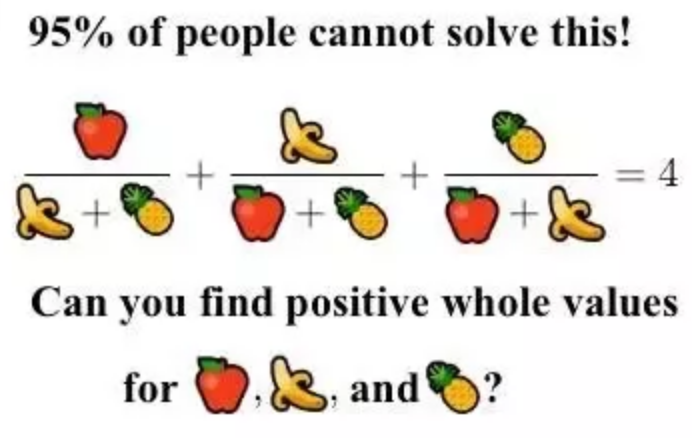
\includegraphics[width=\linewidth, height=1.5in, keepaspectratio]{../figure/elliptic_curve.png}
\caption{Diophantine equations such as finding a positive integer
solution to the equation
\(a(a+b)(a+c)+b(b+a)(b+c)+c(c+a)(c+b)=4(a+b)(a+c)(b+c)\) (depicted more
compactly and whimsically above) can be surprisingly difficult. There
are many equations for which we do not know if they have a solution, and
there is no algorithm to solve them in general. The smallest solution
for this equation has \(80\) digits! See this
\href{https://www.quora.com/How-do-you-find-the-positive-integer-solutions-to-frac-x-y+z-+-frac-y-z+x-+-frac-z-x+y-4}{Quora
post} for more information, including the credits for this image.}
\label{ellipticcurvefig}
\end{marginfigure}

But there are some equations that we simply do not know how to solve
\emph{by any means}. For example, it took more than 200 years until
people succeeded in proving that the equation
\(a^{11} + b^{11} = c^{11}\) has no solution in integers.\footnote{This
  is a special case of what's known as ``Fermat's Last Theorem'' which
  states that \(a^n + b^n = c^n\) has no solution in integers for
  \(n>2\). This was conjectured in 1637 by Pierre de Fermat but only
  proven by Andrew Wiles in 1991. The case \(n=11\) (along with all
  other so called ``regular prime exponents'') was established by Kummer
  in 1850.} The notorious difficulty of so called \emph{Diophantine
equations} (i.e., finding \emph{integer} roots of a polynomial)
motivated the mathematician David Hilbert in 1900 to include the
question of finding a general procedure for solving such equations in
his famous list of twenty-three open problems for mathematics of the
20th century. I don't think Hilbert doubted that such a procedure
exists. After all, the whole history of mathematics up to this point
involved the discovery of ever more powerful methods, and even
impossibility results such as the inability to trisect an angle with a
straightedge and compass, or the non-existence of an algebraic formula
for quintic equations, merely pointed out to the need to use more
general methods.

Alas, this turned out not to be the case for Diophantine equations. In
1970, Yuri Matiyasevich, building on a decades long line of work by
Martin Davis, Hilary Putnam and Julia Robinson, showed that there is
simply \emph{no method} to solve such equations in general:

\hypertarget{MRDP-thm}{}
\begin{theorem}[MRDP Theorem] \label[theorem]{MRDP-thm}

Let \(\ensuremath{\mathit{DIO}}:\{0,1\}^* \rightarrow \{0,1\}\) be the
function that takes as input a string describing a \(100\)-variable
polynomial with integer coefficients \(P(x_0,\ldots,x_{99})\) and
outputs \(1\) if and only if there exists \(z_0,\ldots,z_{99} \in \N\)
s.t. \(P(z_0,\ldots,z_{99})=0\).

Then \(\ensuremath{\mathit{DIO}}\) is uncomputable.

\end{theorem}

As usual, we assume some standard way to express numbers and text as
binary strings. The constant \(100\) is of course arbitrary; the problem
is known to be uncomputable even for polynomials of degree four and at
most 58 variables. In fact the number of variables can be reduced to
nine, at the expense of the polynomial having a larger (but still
constant) degree. See
\href{https://www.jstor.org/stable/2273588}{Jones's paper} for more
about this issue.

\hypertarget{codevsstaticrem}{}
\begin{remark}[Active code vs static data] \label[remark]{codevsstaticrem}

The difficulty in finding a way to distinguish between ``code'' such as
NAND-TM programs, and ``static content'' such as polynomials is just
another manifestation of the phenomenon that \emph{code} is the same as
\emph{data}. While a fool-proof solution for distinguishing between the
two is inherently impossible, finding heuristics that do a reasonable
job keeps many firewall and anti-virus manufacturers very busy (and
finding ways to bypass these tools keeps many hackers busy as well).

\end{remark}

\section{Hardness of quantified integer
statements}\label{Hardness-of-quantified-in}

We will not prove the MRDP Theorem (\cref{MRDP-thm}). However, as we
mentioned, we will prove the uncomputability of
\(\ensuremath{\mathit{QIS}}\) (i.e., \cref{QIS-thm}), which is a special
case of the MRDP Theorem. The reason is that a Diophantine equation is a
special case of a quantified integer statement where the only quantifier
is \(\exists\). This means that deciding the truth of quantified integer
statements is a potentially harder problem than solving Diophantine
equations, and so it is potentially \emph{easier} to prove that
\(\ensuremath{\mathit{QIS}}\) is uncomputable.

\begin{pause} \label[pause]{If-you-find-the-last-sent}

If you find the last sentence confusing, it is worthwhile to reread it
until you are sure you follow its logic. We are so accustomed to trying
to find \emph{solutions} for problems that it can sometimes be hard to
follow the arguments for showing that problems are \emph{uncomputable}.

\end{pause}

Our proof of the uncomputability of \(\ensuremath{\mathit{QIS}}\)
(i.e.~\cref{QIS-thm}) will, as usual, go by reduction from the Halting
problem, but we will do so in two steps:

\begin{enumerate}
\def\labelenumi{\arabic{enumi}.}
\item
  We will first use a reduction from the Halting problem to show that
  deciding the truth of \emph{quantified mixed statements} is
  uncomputable. Quantified mixed statements involve both strings and
  integers. Since quantified mixed statements are a more general concept
  than quantified integer statements, it is \emph{easier} to prove the
  uncomputability of deciding their truth.
\item
  We will then reduce the problem of quantified mixed statements to
  quantifier integer statements.
\end{enumerate}

\subsection{Step 1: Quantified mixed statements and computation
histories}\label{Step--Quantified-mixed-st}

We define \emph{quantified mixed statements} as statements involving not
just integers and the usual arithmetic operators, but also \emph{string
variables} as well.

\hypertarget{QMS-def}{}
\begin{definition}[Quantified mixed statements] \label[definition]{QMS-def}

A \emph{quantified mixed statement} is a well-formed statement with no
unbound variables involving integers, variables, the operators
\(>,<,\times,+,-,=\), the logical operations \(\neg\) (NOT), \(\wedge\)
(AND), and \(\vee\) (OR), as well as quantifiers of the form
\(\exists_{x\in\N}\), \(\exists_{a\in\{0,1\}^*}\), \(\forall_{y\in\N}\),
\(\forall_{b\in\{0,1\}^*}\) where \(x,y,a,b\) are variable names. These
also include the operator \(|a|\) which returns the length of a string
valued variable \(a\), as well as the operator \(a_i\) where \(a\) is a
string-valued variable and \(i\) is an integer valued expression which
is true if \(i\) is smaller than the length of \(a\) and the \(i^{th}\)
coordinate of \(a\) is \(1\), and is false otherwise.

\end{definition}

For example, the true statement that for every string \(a\) there is a
string \(b\) that corresponds to \(a\) in reverse order can be phrased
as the following quantified mixed statement \[
\forall_{a\in\{0,1\}^*} \exists_{b\in \{0,1\}^*}  (|a|=|b|)
\wedge (\forall_{i\in\N} i < |a| \Rightarrow (a_i \Leftrightarrow b_{|a|-i}) \;.
\]

Quantified mixed statements are more general than quantified integer
statements, and so the following theorem is potentially easier to prove
than \cref{QIS-thm}:

\hypertarget{QMS-thm}{}
\begin{theorem}[Uncomputability of quantified mixed statements] \label[theorem]{QMS-thm}

Let \(\ensuremath{\mathit{QMS}}:\{0,1\}^* \rightarrow \{0,1\}\) be the
function that given a (string representation of) a quantified mixed
statement outputs \(1\) if it is true and \(0\) if it is false. Then
\(\ensuremath{\mathit{QMS}}\) is uncomputable.

\end{theorem}

\begin{proofidea} \label[proofidea]{The-idea-behind-the-proof}

The idea behind the proof is similar to that used in showing that
one-dimensional cellular automata are Turing complete
(\cref{onedimcathm}) as well as showing that equivalence (or even
``fullness'') of context free grammars is uncomputable
(\cref{fullnesscfgdef}). We use the notion of a \emph{configuration} of
a NAND-TM program as in \cref{configtmdef}. Such a configuration can be
thought of as a string \(\alpha\) over some large-but-finite alphabet
\(\Sigma\) describing its current state, including the values of all
arrays, scalars, and the index variable \texttt{i}. It can be shown that
if \(\alpha\) is the configuration at a certain step of the execution
and \(\beta\) is the configuration at the next step, then
\(\beta_j = \alpha_j\) for all \(j\) outside of \(\{i-1,i,i+1\}\) where
\(i\) is the value of \texttt{i}. In particular, every value \(\beta_j\)
is simply a function of \(\alpha_{j-1,j,j+1}\). Using these observations
we can write a \emph{quantified mixed statement}
\(\ensuremath{\mathit{NEXT}}(\alpha,\beta)\) that will be true if and
only if \(\beta\) is the configuration encoding the next step after
\(\alpha\). Since a program \(P\) halts on input \(x\) if and only if
there is a sequence of configurations \(\alpha^0,\ldots,\alpha^{t-1}\)
(known as a \emph{computation history}) starting with the initial
configuration with input \(x\) and ending in a halting configuration, we
can define a quantified mixed statement to determine if there is such a
statement by taking a universal quantifier over all strings \(H\) (for
\emph{history}) that encode a tuple
\((\alpha^0,\alpha^1,\ldots,\alpha^{t-1})\) and then checking that
\(\alpha^0\) and \(\alpha^{t-1}\) are valid starting and halting
configurations, and that
\(\ensuremath{\mathit{NEXT}}(\alpha^j,\alpha^{j+1})\) is true for every
\(j\in \{0,\ldots,t-2\}\).

\end{proofidea}

\begin{proof}[Proof of \cref{QMS-thm}] \label[proof]{The-proof-is-obtained-by-}

The proof is obtained by a reduction from the Halting problem.
Specifically, we will use the notion of a \emph{configuration} of a
Turing Machines (\cref{configtmdef}) that we have seen in the context of
proving that one dimensional cellular automata are Turing complete. We
need the following facts about configurations:

\begin{itemize}
\item
  For every Turing Machine \(M\), there is a finite alphabet \(\Sigma\),
  and a \emph{configuration} of \(M\) is a string
  \(\alpha \in \Sigma^*\).
\item
  A configuration \(\alpha\) encodes all the state of the program at a
  particular iteration, including the array, scalar, and index
  variables.
\item
  If \(\alpha\) is a configuration, then
  \(\beta = \ensuremath{\mathit{NEXT}}_P(\alpha)\) denotes the
  configuration of the computation after one more iteration. \(\beta\)
  is a string over \(\Sigma\) of length either \(|\alpha|\) or
  \(|\alpha|+1\), and every coordinate of \(\beta\) is a function of
  just three coordinates in \(\alpha\). That is, for every
  \(j\in \{0,\ldots,|\beta|-1\}\),
  \(\beta_j = \ensuremath{\mathit{MAP}}_P(\alpha_{j-1},\alpha_j,\alpha_{j+1})\)
  where \(\ensuremath{\mathit{MAP}}_P:\Sigma^3 \rightarrow \Sigma\) is
  some function depending on \(P\).
\item
  There are simple conditions to check whether a string \(\alpha\) is a
  valid starting configuration corresponding to an input \(x\), as well
  as to check whether a string \(\alpha\) is a halting configuration. In
  particular these conditions can be phrased as quantified mixed
  statements.
\item
  A program \(M\) halts on input \(x\) if and only if there exists a
  sequence of configurations
  \(H = (\alpha^0,\alpha^1,\ldots,\alpha^{T-1})\) such that \textbf{(i)}
  \(\alpha^0\) is a valid starting configuration of \(M\) with input
  \(x\), \textbf{(ii)} \(\alpha^{T-1}\) is a valid halting configuration
  of \(P\), and \textbf{(iii)}
  \(\alpha^{i+1} = \ensuremath{\mathit{NEXT}}_P(\alpha^i)\) for every
  \(i\in \{0,\ldots,T-2\}\).
\end{itemize}

We can encode such a sequence \(H\) of configuration as a binary string.
For concreteness, we let \(\ell = \lceil \log (|\Sigma|+1) \rceil\) and
encode each symbol \(\sigma\) in \(\Sigma \cup \{ ";" \}\) by a string
in \(\{0,1\}^\ell\). We use ``\(;\)'' as a ``separator'' symbol, and so
encode \(H = (\alpha^0,\alpha^1,\ldots,\alpha^{T-1})\) as the
concatenation of the encodings of each configuration, using ``\(;\)'' to
separate the encoding of \(\alpha^i\) and \(\alpha^{i+1}\) for every
\(i\in [T]\). In particular for every Turing Machine \(M\), \(M\) halts
on the input \(0\) if and only if the following statement \(\varphi_M\)
is true

\[
\exists_{H \in \{0,1\}^*} \text{$H$ encodes halting configuration sequence starting with input $0$} \;.
\]

If we can encode the statement \(\varphi_M\) as a mixed-integer
statement then, since \(\varphi_M\) is true if and only if
\(\ensuremath{\mathit{HALTONZERO}}(M)=1\), this would reduce the task of
computing \(\ensuremath{\mathit{HALTONZERO}}\) to computing
\(\ensuremath{\mathit{MIS}}\), and hence imply (using
\cref{haltonzero-thm} ) that \(\ensuremath{\mathit{MIS}}\) is
uncomputable, completing the proof. Indeed, \(\varphi_M\) can be encoded
as a mixed-integer statement for the following reasons:

\begin{enumerate}
\def\labelenumi{\arabic{enumi}.}
\item
  Let \(\alpha,\beta \in \{0,1\}^*\) be two strings that encode
  configurations of \(M\). We can define a quantified mixed predicate
  \(\ensuremath{\mathit{NEXT}}(\alpha,\beta)\) that is true if and only
  if \(\beta = \ensuremath{\mathit{NEXT}}_M(\beta)\) (i.e., \(\beta\)
  encodes the configuration obtained by proceeding from \(\alpha\) in
  one computational step). Indeed
  \(\ensuremath{\mathit{NEXT}}(\alpha,\beta)\) is true if \textbf{for
  every} \(i \in \{0,\ldots,|\beta|\}\) which is a multiple of \(\ell\),
  \(\beta_{i,\ldots,i+\ell-1} = \ensuremath{\mathit{MAP}}_M(\alpha_{i-\ell,\cdots,i+2\ell-1})\)
  where
  \(\ensuremath{\mathit{MAP}}_M:\{0,1\}^{3\ell} \rightarrow \{0,1\}^\ell\)
  is the finite function above (identifying elements of \(\Sigma\) with
  their encoding in \(\{0,1\}^\ell\)). Since
  \(\ensuremath{\mathit{MAP}}_M\) is a finite function, we can express
  it using the logical operations
  \(\ensuremath{\mathit{AND}}\),\(\ensuremath{\mathit{OR}}\),
  \(\ensuremath{\mathit{NOT}}\) (for example by computing
  \(\ensuremath{\mathit{MAP}}_M\) with
  \(\ensuremath{\mathit{NAND}}\)'s).
\item
  Using the above we can now write the condition that \textbf{for every}
  substring of \(H\) that has the form
  \(\alpha \ensuremath{\mathit{ENC}}(;) \beta\) with
  \(\alpha,\beta \in \{0,1\}^\ell\) and \(\ensuremath{\mathit{ENC}}(;)\)
  being the encoding of the separator ``\(;\)'', it holds that
  \(\ensuremath{\mathit{NEXT}}(\alpha,\beta)\) is true.
\item
  Finally, if \(\alpha^0\) is a binary string encoding the initial
  configuration of \(M\) on input \(0\), checking that the first
  \(|\alpha^0|\) bits of \(H\) equal \(\alpha_0\) can be expressed using
  \(\ensuremath{\mathit{AND}}\),\(\ensuremath{\mathit{OR}}\), and
  \(\ensuremath{\mathit{NOT}}\)'s. Similarly checking that the last
  configuration encoded by \(H\) corresponds to a state in which \(M\)
  will halt can also be expressed as a quantified statement.
\end{enumerate}

Together the above yields a computable procedure that maps every Turing
Machine \(M\) into a quantified mixed statement \(\varphi_M\) such that
\(\ensuremath{\mathit{HALTONZERO}}(M)=1\) if and only if
\(\ensuremath{\mathit{QMS}}(\varphi_M)=1\). This reduces computing
\(\ensuremath{\mathit{HALTONZERO}}\) to computing
\(\ensuremath{\mathit{QMS}}\), and hence the uncomputability of
\(\ensuremath{\mathit{HALTONZERO}}\) implies the uncomputability of
\(\ensuremath{\mathit{QMS}}\).

\end{proof}

\hypertarget{alternativeproofs}{}
\begin{remark}[Alternative proofs] \label[remark]{alternativeproofs}

There are several other ways to show that \(\ensuremath{\mathit{QMS}}\)
is uncomputable. For example, we can express the condition that a
1-dimensional cellular automaton eventually writes a ``\(1\)'' to a
given cell from a given initial configuration as a quantified mixed
statement over a string encoding the history of all configurations. We
can then use the fact that cellular automatons can simulate Turing
machines (\cref{onedimcathm}) to reduce the halting problem to
\(\ensuremath{\mathit{QMS}}\). We can also use other well known
uncomputable problems such as tiling or the
\href{https://en.wikipedia.org/wiki/Post_correspondence_problem}{post
correspondence problem}. \cref{postcorrespondenceproblemex} and
\cref{puzzleex} explore two alternative proofs of \cref{QMS-thm}.

\end{remark}

\subsection{Step 2: Reducing mixed statements to integer
statements}\label{Step--Reducing-mixed-stat}

We now show how to prove \cref{QIS-thm} using \cref{QMS-thm}. The idea
is again a proof by reduction. We will show a transformation of every
quantifier mixed statement \(\varphi\) into a quantified \emph{integer}
statement \(\xi\) that does not use string-valued variables such that
\(\varphi\) is true if and only if \(\xi\) is true.

To remove string-valued variables from a statement, we encode every
string by a pair integer. We will show that we can encode a string
\(x\in \{0,1\}^*\) by a pair of numbers \((X,n)\in \N\) s.t.

\begin{itemize}
\item
  \(n=|x|\)
\item
  There is a quantified integer statement
  \(\ensuremath{\mathit{COORD}}(X,i)\) that for every \(i<n\), will be
  true if \(x_i=1\) and will be false otherwise.
\end{itemize}

This will mean that we can replace a ``for all'' quantifier over strings
such as \(\forall_{x\in \{0,1\}^*}\) with a pair of quantifiers over
\emph{integers} of the form \(\forall_{X\in \N}\forall_{n\in\N}\) (and
similarly replace an existential quantifier of the form
\(\exists_{x\in \{0,1\}^*}\) with a pair of quantifiers
\(\exists_{X\in \N}\exists_{n\in\N}\)) . We can then replace all calls
to \(|x|\) by \(n\) and all calls to \(x_i\) by
\(\ensuremath{\mathit{COORD}}(X,i)\). This means that if we are able to
define \(\ensuremath{\mathit{COORD}}\) via a quantified integer
statement, then we obtain a proof of \cref{QIS-thm}, since we can use it
to map every mixed quantified statement \(\varphi\) to an equivalent
quantified integer statement \(\xi\) such that \(\xi\) is true if and
only if \(\varphi\) is true, and hence
\(\ensuremath{\mathit{QMS}}(\varphi)=\ensuremath{\mathit{QIS}}(\xi)\).
Such a procedure implies that the task of computing
\(\ensuremath{\mathit{QMS}}\) reduces to the task of computing
\(\ensuremath{\mathit{QIS}}\), which means that the uncomputability of
\(\ensuremath{\mathit{QMS}}\) implies the uncomputability of
\(\ensuremath{\mathit{QIS}}\).

The above shows that proof of \cref{QIS-thm} all boils down to finding
the right encoding of strings as integers, and the right way to
implement \(\ensuremath{\mathit{COORD}}\) as a quantified integer
statement. To achieve this we use the following technical result :

\hypertarget{primeseq}{}
\begin{lemma}[Constructible prime sequence] \label[lemma]{primeseq}

There is a sequence of prime numbers \(p_0 < p_1 < p_2 < \cdots\) such
that there is a quantified integer statement
\(\ensuremath{\mathit{PSEQ}}(p,i)\) that is true if and only if
\(p=p_i\).

\end{lemma}

Using \cref{primeseq} we can encode a \(x\in\{0,1\}^*\) by the numbers
\((X,n)\) where \(X = \prod_{x_i=1} p_i\) and \(n=|x|\). We can then
define the statement \(\ensuremath{\mathit{COORD}}(X,i)\) as \[
\ensuremath{\mathit{COORD}}(X,i) = \exists_{p\in\N}  \ensuremath{\mathit{PSEQ}}(p,i) \wedge \ensuremath{\mathit{DIVIDES}}(p,X) 
\] where \(\ensuremath{\mathit{DIVIDES}}(a,b)\), as before, is defined
as \(\exists_{c\in\N} a\times c = b\). Note that indeed if \(X,n\)
encodes the string \(x\in \{0,1\}^*\), then for every \(i<n\),
\(\ensuremath{\mathit{COORD}}(X,i)=x_i\), since \(p_i\) divides \(X\) if
and only if \(x_i=1\).

Thus all that is left to conclude the proof of \cref{QIS-thm} is to
prove \cref{primeseq}, which we now proceed to do.

\begin{proof} \label[proof]{The-sequence-of-prime-num}

The sequence of prime numbers we consider is the following: We fix \(C\)
to be a sufficiently large constant (\(C=2^{2^{34}}\)
\href{https://arxiv.org/pdf/1401.4233.pdf}{will do}) and define \(p_i\)
to be the smallest prime number that is in the interval
\([(i+C)^3+1,(i+C+1)^3-1]\). It is known that there exists such a prime
number for every \(i\in\N\). Given this, the definition of
\(\ensuremath{\mathit{PSEQ}}(p,i)\) is simple: \[
(p > (i+C)\times (i+C)\times (i+C)  ) \wedge (p < (i+C+1)\times(i+C+1)\times (i+C+1) )\wedge
\left(\forall_{p'} \neg \ensuremath{\mathit{PRIME}}(p') \vee (p' \leq i) \vee (p' \geq p) \right) \;,
\] We leave it to the reader to verify that
\(\ensuremath{\mathit{PSEQ}}(p,i)\) is true iff \(p=p_i\).

\end{proof}

To sum up we have shown that for every quantified mixed statement
\(\varphi\), we can compute a quantified integer statement \(\xi\) such
that \(\ensuremath{\mathit{QMS}}(\varphi)=1\) if and only if
\(\ensuremath{\mathit{QIS}}(\xi)=1\). Hence the uncomputability of
\(\ensuremath{\mathit{QMS}}\) (\cref{QMS-thm}) implies the
uncomputability of \(\ensuremath{\mathit{QIS}}\), completing the proof
of \cref{QIS-thm}, and so also the proof of Gödel's Incompleteness
Theorem for quantified integer statements (\cref{godelthmqis}).

\begin{recap} \label[recap]{Uncomputable-functions-in}

\begin{itemize}
\tightlist
\item
  Uncomputable functions include also functions that seem to have
  nothing to do with NAND-TM programs or other computational models such
  as determining the satisfiability of diophantine equations.
\item
  This also implies that for any sound proof system (and in particular
  every finite axiomatic system) \(S\), there are interesting statements
  \(X\) (namely of the form ``\(F(x)=0\)'' for an uncomputable function
  \(F\)) such that \(S\) is not able to prove either \(X\) or its
  negation.
\end{itemize}

\end{recap}

\section{Exercises}\label{Exercises}

\hypertarget{godelfromqisex}{}
\begin{exercise}[Gödel's Theorem from uncomputability of $QIS$] \label[exercise]{godelfromqisex}

Prove \cref{godelthmqis} using \cref{QIS-thm}

\end{exercise}

\hypertarget{proofsanduncomputex}{}
\begin{exercise}[Proof systems and uncomputability] \label[exercise]{proofsanduncomputex}

Let \(\ensuremath{\mathit{FINDPROOF}}:\{0,1\}^* \rightarrow \{0,1\}\) be
the following function. On input a Turing machine \(V\) (which we think
of as the verifying algorithm for a proof system) and a string
\(x\in \{0,1\}^*\), \(\ensuremath{\mathit{FINDPROOF}}(V,x)=1\) if and
only if there exists \(w\in \{0,1\}^*\) such that \(V(x,w)=1\).

\begin{enumerate}
\def\labelenumi{\arabic{enumi}.}
\item
  Prove that \(\ensuremath{\mathit{FINDPROOF}}\) is uncomputable.
\item
  Prove that there exists a Turing machine \(V\) such that \(V\)
  \emph{halts on every input \(x,v\)} but the function
  \(\ensuremath{\mathit{FINDPROOF}}_V\) defined as
  \(\ensuremath{\mathit{FINDPROOF}}_V(x) = \ensuremath{\mathit{FINDPROOF}}(V,x)\)
  is uncomputable. See footnote for hint.\footnote{\emph{Hint:} think of
    \(x\) as saying ``Turing Machine \(M\) halts on input \(u\)'' and
    \(w\) being a proof that is the number of steps that it will take
    for this to happen. Can you find an always-halting \(V\) that will
    verify such statements?}
\end{enumerate}

\end{exercise}

\hypertarget{floorexpressionex}{}
\begin{exercise}[Expression for floor] \label[exercise]{floorexpressionex}

Let
\(\ensuremath{\mathit{FSQRT}}(n,m) = \forall_{j \in \N} ((j \times j)>m) \vee (j \leq n)\).
Prove that \(\ensuremath{\mathit{FSQRT}}(n,m)\) is true if and only if
\(n =\floor{\sqrt{m}}\).

\end{exercise}

\hypertarget{godelthemex}{}
\begin{exercise}[axiomatic proof systems] \label[exercise]{godelthemex}

For every representation of logical statements as strings, we can define
an axiomatic proof system to consist of a finite set of strings \(A\)
and a finite set of rules \(I_0,\ldots,I_{m-1}\) with
\(I_j: (\{0,1\}^*)^{k_j} \rightarrow \{0,1\}^*\) such that a proof
\((s_1,\ldots,s_n)\) that \(s_n\) is true is valid if for every \(i\),
either \(s_i \in A\) or is some \(j\in [m]\) and are
\(i_1,\ldots,i_{k_j} < i\) such that
\(s_i = I_j(s_{i_1},\ldots,i_{k_j})\). A system is \emph{sound} if
whenever there is no false \(s\) such that there is a proof that \(s\)
is true Prove that for every uncomputable function
\(F:\{0,1\}^* \rightarrow \{0,1\}\) and every sound axiomatic proof
system \(S\) (that is characterized by a finite number of axioms and
inference rules), there is some input \(x\) for which the proof system
\(S\) is not able to prove neither that \(F(x)=0\) nor that
\(F(x) \neq 0\).

\end{exercise}


\begin{marginfigure}
\centering
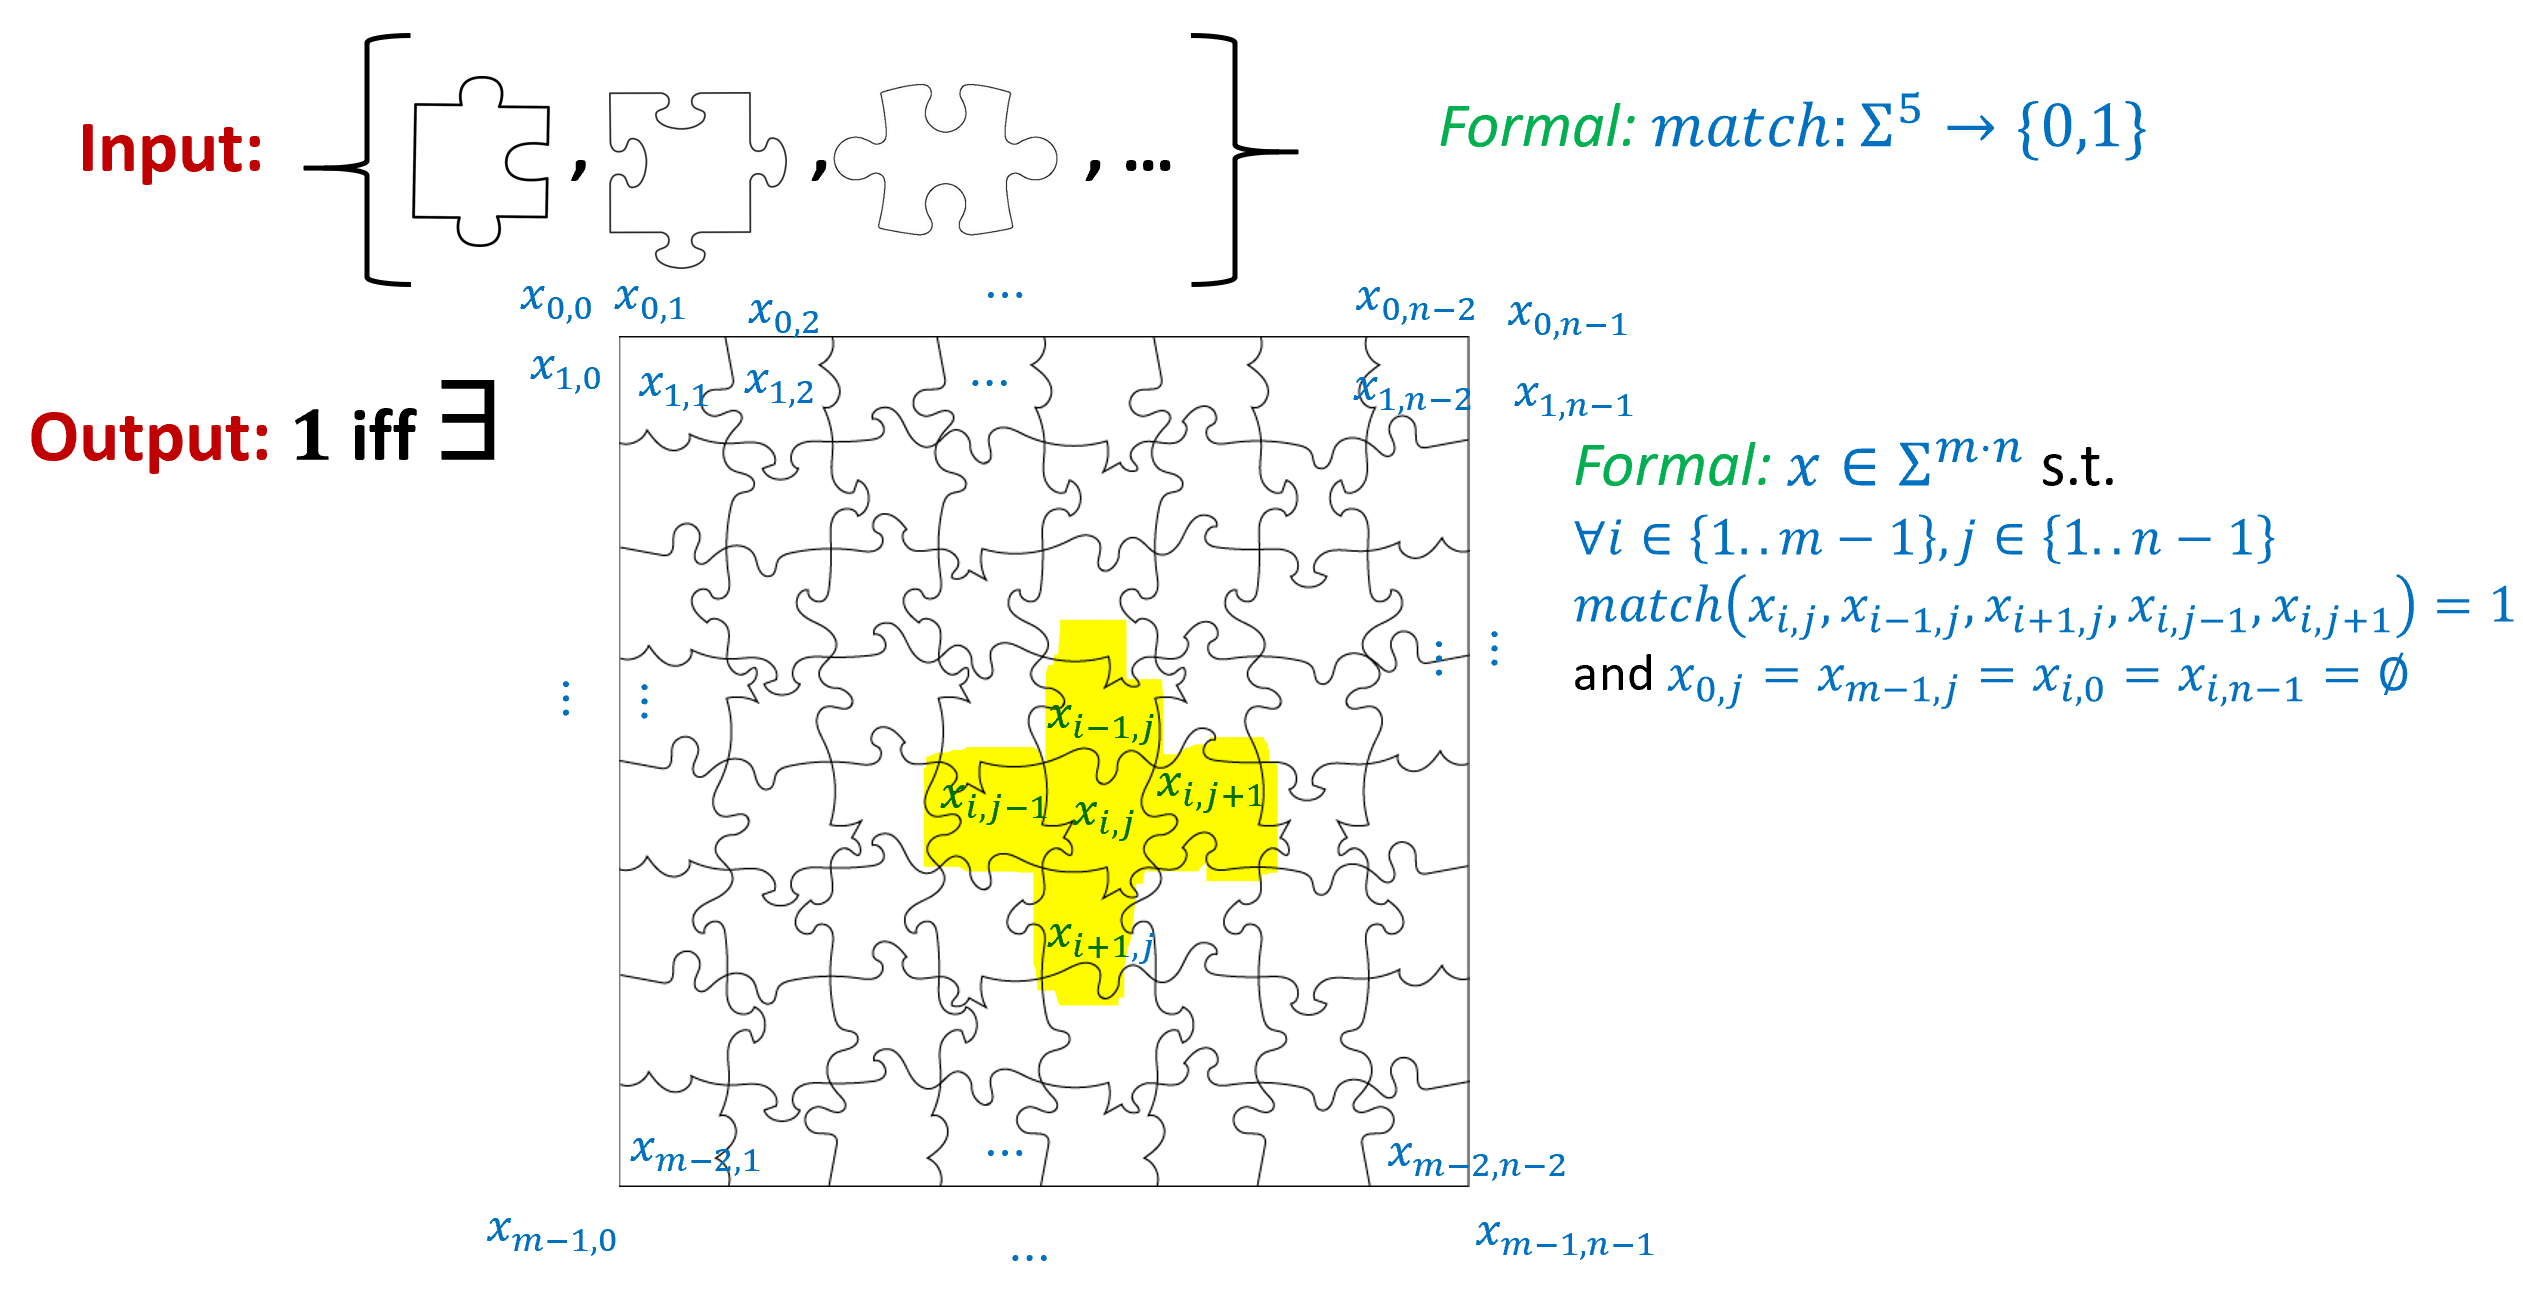
\includegraphics[width=\linewidth, height=1.5in, keepaspectratio]{../figure/puzzleprob.png}
\caption{In the \emph{puzzle problem}, the input can be thought of as a
finite collection \(\Sigma\) of \emph{types of puzzle pieces} and the
goal is to find out whether or not find a way to arrange pieces from
these types in a rectangle. Formally, we model the input as a pair of
functions
\(match_{\leftrightarrow},match_{\updownarrow}:\Sigma^2 \rightarrow \{0,1\}\)
that such that \(match_{\leftrightarrow}(left,right)=1\) (respectively
\(match_{\updownarrow}(up,down)=1\) ) if the pair of pieces are
compatible when placed in their respective positions. We assume
\(\Sigma\) contains a special symbol \(\varnothing\) corresponding to
having no piece, and an arrangement of puzzle pieces by an
\((m-2)\times(n-2)\) rectangle is modeled by a string
\(x\in \Sigma^{m\cdot n}\) whose ``outer coordinates'' are \(\emptyset\)
and such that for every \(i \in [n-1],j \in [m-1]\),
\(match_{\updownarrow}(x_{i,j},x_{i+1,j})=1\) and
\(match_{\leftrightarrow}(x_{i,j},x_{i,j+1})=1\).}
\label{puzzleprobfig}
\end{marginfigure}

\hypertarget{postcorrespondenceproblemex}{}
\begin{exercise}[Post Corrrespondence Problem] \label[exercise]{postcorrespondenceproblemex}

In the
\href{https://en.wikipedia.org/wiki/Post_correspondence_problem}{Post
Correspondence Problem} the input is a set
\(S = \{ (\alpha^0,\beta^0), \ldots, (\beta^{c-1},\beta^{c-1}) \}\)
where each \(\alpha^i\) and \(\beta^j\) is a string in \(\{0,1\}^*\). We
say that \(\ensuremath{\mathit{PCP}}(S)=1\) if and only if there exists
a list \((\alpha_0,\beta_0),\ldots,(\alpha_{n-1},\beta_{n-1})\) of pairs
in \(S\) such that \[
\alpha_0 \alpha_1 \cdots \alpha_{m-1} = \beta_0 \beta_1 \cdots \beta_{m-1} \;.
\] (We can think of each pair \((\alpha,\beta) \in S\) as a ``domino
tile'' and the question is whether we can stack a list of such tiles so
that the top and the bottom yield the same string.) It can be shown that
the \(\ensuremath{\mathit{PCP}}\) is uncomputable by a fairly
straightforward though somewhat tedious proof (see for example the
Wikipedia page for the Post Correspondence Problem or Section 5.2 in
\cite{SipserBook}).

Use this fact to provide a direct proof that
\(\ensuremath{\mathit{QMS}}\) is uncomputable by showing that there
exists a computable map \(R:\{0,1\}^* \rightarrow \{0,1\}^*\) such that
\(\ensuremath{\mathit{PCP}}(S) = \ensuremath{\mathit{QMS}}(R(S))\) for
every string \(S\) encoding an instance of the post correspondence
problem.

\end{exercise}

\hypertarget{puzzleex}{}
\begin{exercise}[Uncomputability of puzzle] \label[exercise]{puzzleex}

Let \(\ensuremath{\mathit{PUZZLE}}:\{0,1\}^* \rightarrow \{0,1\}\) be
the problem of determining, given a finite collection of types of
``puzzle pieces'', whether it is possible to put them together in a
rectangle, see \cref{puzzleprobfig}. Formally, we think of such a
collection as a finite set \(\Sigma\) (see \cref{puzzleprobfig}). We
model the criteria as to which pieces ``fit together'' by a pair of
finite function
\(match_{\updownarrow}, match_{\leftrightarrow}:\Sigma^2 \rightarrow \{0,1\}\)
such that a piece \(a\) fits above a piece \(b\) if and only if
\(match_{\updownarrow}(a,b)=1\) and a piece \(c\) fits to the left of a
piece \(d\) if and only if \(match_{\leftrightarrow}(c,d)=1\). To model
the ``straight edge'' pieces that can be placed next to a ``blank spot''
we assume that \(\Sigma\) contains the symbol \(\varnothing\) and the
matching functions are defined accordingly. A \emph{square tiling} of
\(\Sigma\) is an \(m\times n\) long string \(x \in \Sigma^{mn}\), such
that for every \(i\in \{1,\ldots,m-2 \}\) and
\(j\in \{1,\ldots,n-2 \}\),
\(match(x_{i,j},x_{i-1,j},x_{i+1,j},x_{i,j-1},x_{i,j+1})=1\) (i.e.,
every ``internal pieve'' fits in with the pieces adjacent to it). We
also require all of the ``outer pieces'' (i.e., \(x_{i,j}\) where
\(i\in \{0,m-1\}\) of \(j\in \{0,n-1\}\)) are ``blank'' or equal to
\(\varnothing\). The function \(\ensuremath{\mathit{PUZZLE}}\) takes as
input a string describing the set \(\Sigma\) and the function \(match\)
and outputs \(1\) if and only if there is some square tiling of
\(\Sigma\): some not all blank string \(x\in \Sigma^{mn}\) satisfying
the above condition.

\begin{enumerate}
\def\labelenumi{\arabic{enumi}.}
\item
  Prove that \(\ensuremath{\mathit{PUZZLE}}\) is uncomputable.
\item
  Give a reduction from \(\ensuremath{\mathit{PUZZLE}}\) to
  \(\ensuremath{\mathit{QMS}}\).
\end{enumerate}

\end{exercise}

\hypertarget{MRDPexe}{}
\begin{exercise}[MRDP exercise] \label[exercise]{MRDPexe}

The MRDP theorem states that the problem of determining, given a
\(k\)-variable polynomial \(p\) with integer coefficients, whether there
exists integers \(x_0,\ldots,x_{k-1}\) such that
\(p(x_0,\ldots,x_{k-1})=0\) is uncomputable. Consider the following
\emph{quadratic integer equation problem}: the input is a list of
polynomials \(p_0,\ldots,p_{m-1}\) over \(k\) variables with integer
coefficients, where each of the polynomials is of degree at most two
(i.e., it is a \emph{quadratic} function). The goal is to determine
whether there exist integers \(x_0,\ldots,x_{k-1}\) that solve the
equations \(p_0(x)= \cdots = p_{m-1}(x)=0\).

Use the MRDP Theorem to prove that this problem is uncomputable. That
is, show that the function
\(\ensuremath{\mathit{QUADINTEQ}}:\{0,1\}^* \rightarrow \{0,1\}\) is
uncomputable, where this function gets as input a string describing the
polynomials \(p_0,\ldots,p_{m-1}\) (each with integer coefficients and
degree at most two), and outputs \(1\) if and only if there exists
\(x_0,\ldots,x_{k-1} \in \mathbb{Z}\) such that for every \(i\in [m]\),
\(p_i(x_0,\ldots,x_{k-1})=0\). See footnote for hint\footnote{You can
  replace the equation \(y=x^4\) with the pair of equations \(y=z^2\)
  and \(z=x^2\). Also, you can replace the equation \(w = x^6\) with the
  three equations \(w=yu\), \(y = x^4\) and \(u=x^2\).}

\end{exercise}

\hypertarget{buseybeaverex}{}
\begin{exercise}[The Busy Beaver problem] \label[exercise]{buseybeaverex}

In this question we define the NAND-TM variant of the
\href{https://www.scottaaronson.com/writings/bignumbers.html}{busy
beaver function}.

\begin{enumerate}
\def\labelenumi{\arabic{enumi}.}
\item
  We define the function \(T:\{0,1\}^* \rightarrow \mathbb{N}\) as
  follows: for every string \(P\in \{0,1\}^*\), if \(P\) represents a
  NAND-TM program such that when \(P\) is executed on the input \(0\)
  (i.e., the string of length 1 that is simply \(0\)), a total of \(M\)
  lines are executed before the program halts, then \(T(P)=M\).
  Otherwise (if \(P\) does not represent a NAND-TM program, or it is a
  program that does not halt on \(0\)), \(T(P)=0\). Prove that \(T\) is
  uncomputable.
\item
  Let \(\ensuremath{\mathit{TOWER}}(n)\) denote the number
  \(\underbrace{2^{2^{2^{{\iddots}^2}}}}_{n\text{ times}}\) (that is, a
  ``tower of powers of two'' of height \(n\)). To get a sense of how
  fast this function grows, \(\ensuremath{\mathit{TOWER}}(1)=2\),
  \(\ensuremath{\mathit{TOWER}}(2)=2^2=4\),
  \(\ensuremath{\mathit{TOWER}}(3)=2^{2^2}=16\),
  \(\ensuremath{\mathit{TOWER}}(4) = 2^{16} = 65536\) and
  \(\ensuremath{\mathit{TOWER}}(5) = 2^{65536}\) which is about
  \(10^{20000}\). \(\ensuremath{\mathit{TOWER}}(6)\) is already a number
  that is too big to write even in scientific notation. Define
  \(\ensuremath{\mathit{NBB}}:\mathbb{N} \rightarrow \mathbb{N}\) (for
  ``NAND-TM Busy Beaver'') to be the function
  \(\ensuremath{\mathit{NBB}}(n) = \max_{P\in \{0,1\}^n} T(P)\) where
  \(T:\mathbb{N} \rightarrow \mathbb{N}\) is the function defined in
  Item 1. Prove that \(\ensuremath{\mathit{NBB}}\) grows \emph{faster}
  than \(\ensuremath{\mathit{TOWER}}\), in the sense that
  \(\ensuremath{\mathit{TOWER}}(n) = o(\ensuremath{\mathit{NBB}}(n))\)
  (i.e., for every \(\epsilon>0\), there exists \(n_0\) such that for
  every \(n>n_0\),
  \(\ensuremath{\mathit{TOWER}}(n) < \epsilon \cdot \ensuremath{\mathit{NBB}}(n)\).).\footnote{You
    will not need to use very specific properties of the
    \(\ensuremath{\mathit{TOWER}}\) function in this exercise. For
    example, \(\ensuremath{\mathit{NBB}}(n)\) also grows faster than the
    \href{https://en.wikipedia.org/wiki/Ackermann_function}{Ackerman
    function}. You might find
    \href{https://www.scottaaronson.com/blog/?p=3445}{Aaronson's blog
    post} on the same topic to be quite interesting, and relevant to
    this book at large. If you like it then you might also enjoy
    \href{https://terrytao.wordpress.com/2010/10/10/the-cosmic-distance-ladder-ver-4-1/}{this
    piece by Terence Tao}.}
\end{enumerate}

\end{exercise}

\section{Bibliographical notes}\label{Bibliographical-notes}

As mentioned before, Gödel, Escher, Bach \cite{hofstadter1999} is a
highly recommended book covering Gödel's Theorem. A classic popular
science book about Fermat's Last Theorem is \cite{singh1997fermat}.

Cantor's are used for both Turing and Gödel's theorems. In a twist of
fate, using techniques originating from the works of Gödel and Turing,
Paul Cohen showed in 1963 that Cantor's \emph{Continuum Hypothesis} is
independent of the axioms of set theory, which means that neither it nor
its negation is provable from these axioms and hence in some sense can
be considered as ``neither true nor false'' (see \cite{cohen2008set}).
The \href{https://goo.gl/9ieBVq}{Continuum Hypothesis} is the conjecture
that for every subset \(S\) of \(\mathbb{R}\), either there is a
one-to-one and onto map between \(S\) and \(\N\) or there is a
one-to-one and onto map between \(S\) and \(\mathbb{R}\). It was
conjectured by Cantor and listed by Hilbert in 1900 as one of the most
important problems in mathematics. See also the non-conventional survey
of Shelah \cite{shelah2003logical}. See
\href{https://gowers.wordpress.com/2017/09/19/two-infinities-that-are-surprisingly-equal/}{here}
for recent progress on a related question.

Thanks to Alex Lombardi for pointing out an embarrassing mistake in the
description of Fermat's Last Theorem. (I said that it was open for
exponent 11 before Wiles' work.)
